


\documentclass{article}[12pt]
\usepackage{fullpage,graphicx, setspace, latexsym, cite,amsmath,amssymb,color,subfigure}
%\usepackage{epstopdf}
%\DeclareGraphicsExtensions{.pdf,.eps,.png,.jpg,.mps} 
\usepackage{amssymb} %maths
\usepackage{amsmath} %maths
\usepackage{amsthm}
\usepackage{hyperref}
\usepackage{enumitem}
\usepackage{bm}
\bibliographystyle{unsrt}

\newtheorem{theorem}{Theorem}
\newtheorem{prop}{Proposition}
\newtheorem{corollary}{Corollary}
\newtheorem{lemma}{Lemma}
\newtheorem{defn}{Definition}
\newtheorem{ex}{Example}
\usepackage{float}

\def\R{\mathbb{R}}
\def\Eps{\mathcal{E}}
\def\E{\E}
\def\V{\mathbb{V}}
\def\F{\mathcal{F}}
\def\G{\mathcal{G}}
\def\H{\mathcal{H}}
\def\S{\mathcal{S}}
\def\P{\mathbb{P}}
\def\1{\mathbf{1}}
\def\n{\nappa}
\def\h{\mathbf{w}}
\def\v{\mathbf{v}}
\def\x{\mathbf{x}}
\def\X{\mathcal{X}}
\def\Y{\mathcal{Y}}
\def\eps{\epsilon}
\def\y{\mathbf{y}}
\def\e{\mathbf{e}}
\newcommand{\norm}[1]{\left|\left|#1\right|\right|}
\DeclareMathOperator*{\argmin}{arg\,min}
\DeclareMathOperator*{\argmax}{arg\,max}

\newcommand{\lecture}[4]{
   \pagestyle{myheadings}
   \thispagestyle{plain}
   \newpage
   % \setcounter{lecnum}{#1}
   \setcounter{page}{1}
   \setlength{\headsep}{10mm}
   \noindent
   \begin{center}
   \framebox{
      \vbox{\vspace{2mm}
    \hbox to 6.28in { {\bf ESE 680-004: Learning and Control
   \hfill Fall 2019} }
       \vspace{4mm}
       \hbox to 6.28in { {\Large \hfill Lecture #1: #2  \hfill} }
       \vspace{2mm}
       \hbox to 6.28in { {\it Lecturer: #3 \hfill Scribes: #4} }
      \vspace{2mm}}
   }
   \end{center}
   \markboth{Lecture #1: #2}{Lecture #1: #2}

   \noindent{\bf Disclaimer}: {\it These notes have not been subjected to the
   usual scrutiny reserved for formal publications. }
   \vspace*{4mm}
}

%notation

\def \E{\mathbb E}
\def \P{\mathbb P}
\def \R{\mathbb R}
\def \A{\cal A}
\newcommand{\cov}{\mathrm{cov}}
\DeclareMathOperator{\Tr}{Tr}

\newcommand*\diff{\mathop{}\!\mathrm{d}}
\newtheorem{definition}{Definition}
\newtheorem{example}{Example}



\begin{document}

\lecture{24}{Gaussian Processes}{Nikolai Matni}{Al\"ena Rodionova}

\section{Preliminaries}
\subsection{Gaussian Random Vectors}
\begin{definition}
	Random vector $x\in\mathbb{R}^n$ is \textbf{Gaussian} if it has density
	\begin{equation}
	\label{eq:gaus_var}
	p_x(v)=\frac{1}{\sqrt{(2\pi)^n \det(\Sigma)}} \exp
	\left(
	-\frac{1}{2} (v-\mu)^\top \Sigma^{-1}(v-\mu)
	\right)
	\end{equation}
for some $\Sigma=\Sigma^\top \succ 0$, and $\mu\in\mathbb{R}^n$.
\end{definition}
We will write a Gaussian random vector as:
\begin{equation*}
x\sim\mathcal{N}(\mu,\Sigma).
\end{equation*}

Vector $\mu\in\mathbb{R}^n$ is the \textit{mean} or \textit{expected value} of $x$ and is defined as
\begin{equation}
\mu = \E x = \int v p_x(v) \diff v
\end{equation}
and the matrix $\Sigma$ is the \textit{covariance matrix} of $x$, given dy
\begin{equation}
\Sigma = \E\left[(x-\mu)(x-\mu)^\top\right] = \E [xx^\top] - 
\E x \mu^\top - \mu \E x^\top + \mu \mu^\top = 
\E [xx^\top] - \mu \mu^\top
= \int v p_x(v) \diff v
\end{equation}
Variables $\mu$ and $\Sigma$ determine the shape of density.
Graphical representation of the probability density function for $x\sim \mathcal{N}(0, 1)$ is given in a Figure~\ref{fig:st_normal}.

\begin{figure}[h]
	\centering
	\includegraphics[width=0.4\textwidth]{figures/st_normal.png}
	\caption{\small Probability density function for $x\sim \mathcal{N}(0, 1)$.}
	\vspace{-10pt}
	\label{fig:st_normal}
\end{figure}

\begin{example}
$x\sim\mathcal{N}(0,I)$ means $x_i$ are independent identically distributed (IID) random variables $\mathcal{N}(0,1)$. 
\end{example}

\begin{definition}
	Mean (norm) square deviation of $x$ from $\mu$ is\footnote{Using $\Tr AB = \Tr BA$.}
	\begin{equation}
	\E ||x-\mu||^2 = \E \Tr(x-\mu)(x-\mu)^\top = \Tr \Sigma = \sum\limits_{i=1}^{n} \Sigma_{ii}
	\end{equation}
\end{definition}

%%%%%%%%%%%%%%%%%%%%%%%%%%%%%%%%%%%%%%%%%%%%%%%%%%
\subsection{Confidence Ellipsoids}
Using Equation~\eqref{eq:gaus_var} it is easy to show that $p_x(v)$ is constant for $(v-\mu)^\top \Sigma^{-1} (v-\mu)=\alpha$, i.e., on the surface of the ellipsoid
\begin{equation}
\label{eq:eps}
\Eps_\alpha := \{v\ |\ (v-\mu)^\top \Sigma^{-1} (v-\mu)\leq \alpha\}.
\end{equation}
\begin{definition}
$\eta$-confidence set for random variable $z$ is  the smallest volume set $S$ such that
\begin{equation}
\P\left[z\in S\right]\geq \eta.
\end{equation} 
\end{definition}
\begin{definition}[Confidence Ellipsoids]
	\label{def:conf_el}
	For Gaussian random variables, the $\Eps_\alpha$ are the $\eta$-confidence sets (using Equation~\eqref{eq:eps}), and are called \textbf{confidence ellipsoids}, where $\alpha$ determines confidence level $\eta$.
\end{definition}
Mean $\mu$ gives the center of the ellipsoid $\Eps_\alpha$, and semiaxes are defined as $\sqrt{\alpha \lambda_i}u_i$, where $u_i$ are orthonormal eigenvectors of $\Sigma$ with eigenvalues $\lambda_i$. 

\subsubsection{Confidence Levels}
Notice that since $x$ is a Gaussian random variable and $\Sigma\succ 0$, the non-negative random variable $(x-\mu)^\top \Sigma^{-1} (x-\mu)$ has a $\chi_n^2$ distribution\footnote{Chi-squared distribution $\chi_n^2$ is the distribution of a sum of the squares of $n$ independent standard normal random variables,  \url{https://en.wikipedia.org/wiki/Chi-squared_distribution}}, with a CDF $F_{\chi_n^2}(\alpha)$. Hence, using the above confidence ellipsoid's definition~\ref{def:conf_el},  $\mathbb{P}\left[x\in\Eps_\alpha\right]=F_{\chi_n^2}(\alpha)$.

Some good approximations are:
\begin{itemize}[noitemsep,topsep=0pt]
	\item $\Eps_n$ gives about $50\%$ of probability mass.
	\item $\Eps_{n+2\sqrt{n}}$ gives about $90\%$ of probability mass.
\end{itemize}

\begin{example}
	Let $x\sim\mathcal{N}(\mu,\Sigma)$ with $\mu=\begin{bmatrix}
	2\\1 
	\end{bmatrix}$ and $\Sigma=\begin{bmatrix}
	2 &1\\ 1 &1
	\end{bmatrix}$. Then $90\%$ confidence ellipsoid corresponds to $\alpha=4.6$, see Figure~\ref{fig:ex_el}. In this experiment, 91 out of 100 samples fall in $\Eps_{4.6}$.
\end{example}
\begin{figure}[h]
	\centering
	\includegraphics[width=0.4\textwidth]{figures/ex_el.png}
	\caption{\small Confidence ellipsoid $\Eps_\alpha$ for $\alpha=4.6$.}
	\vspace{-10pt}
	\label{fig:ex_el}
\end{figure}


\subsection{Affine Transformations}
Suppose that $x\sim\mathcal{N}(\mu,\Sigma_x)$. Consider an affine transformation of $x$: $z=Ax+b$, where $A\in\mathbb{R}^{m\times n}$, $b\in\mathbb{R}^m$. Then $z$ is Gaussian with mean
\begin{equation}
\bar{z}=\E z=\E (Ax+b)= A\E x +b = A\mu +b,
\end{equation}
and covariance
\begin{equation}
\begin{aligned}
\Sigma_z &= \E \left[ (z-\bar{z})(z-\bar{z})^\top \right]=\\
&=\E \left[(Ax+b - A\mu-b)(Ax+b - A\mu-b)^\top \right] = \\
&=A\E \left[(x-\mu)(x-\mu)\top\right]A^\top =\\
&= A\Sigma_x A^\top 
\end{aligned}
\end{equation}
\begin{example}
	For $w\sim\mathcal{N}(0,I)$ and $x=\Sigma^{1/2}w +\mu$, we have $x\sim\mathcal{N}(\mu,\Sigma)$.
	Useful for simulating vectors with given mean and covariance
\end{example}
\begin{example}
	Conversely, for $x\sim\mathcal{N}(\mu,\Sigma)$ and $z=\Sigma^{-1/2}(x-\mu)$, we have $x\sim\mathcal{N}(0,I)$. So it normalizes and decorrelates. Called \textit{whitening} or \textit{normalizing}.
\end{example}
\begin{example}
	For $x\sim\mathcal{N}(\mu,\Sigma)$ and $c\in\mathbb{R}^n$ scalar $c^\top x\sim\mathcal{N}(c^\top\mu,\,c^\top \Sigma c)$.
	This means that we can identify unit length direction of minimum (maximum) variability for $x$ by selecting the orthonormal eigenvector $u$ corresponding to the minimum (maximum) eigenvalue $\lambda_{\min}$ ($\lambda_{\max}$)of $\Sigma$:
	\begin{equation}
	\Sigma u = \lambda u,\quad ||u||=1.
	\end{equation}
	Standard deviation of $u_n^\top x$ is $\sqrt{\lambda_{\min}}$.
\end{example}
\subsection{Linear Measurements}
Suppose that we obtain liear measurements with noise $y=Ax+v$,
where $x\in\mathbb{R}^n$ is what we want to estimate, $y\in\mathbb{R}^m$ is a measurement, $A\in\mathbb{R}^{m\times n}$ characterizes sensors or measurements and $v$ is a sensor noise. We also assume that $x\sim\mathcal{N}(\bar{x},\,\Sigma_x)$, so the \textit{prior distribution} of $x$ that describes initial uncertainty
about $x$ is given. Another assumption is $v\sim\mathcal{N}(\bar{v},\,\Sigma_v)$, where $\bar{v}$ is noise \textit{bias} or \textit{offset} and $\Sigma_v$ is noise covariance. $x$ and $v$ are assumed to be independent.
Then we have
\begin{equation}
\begin{bmatrix}
x\\v
\end{bmatrix}
\sim\mathcal{N}
\left(
\begin{bmatrix}
\bar{x}\\\bar{v}
\end{bmatrix},\ 
\begin{bmatrix}
\Sigma_x & \\
& \Sigma_v
\end{bmatrix}
\right).
\end{equation}
We can write
\begin{equation}
\E \begin{bmatrix}
x \\ y
\end{bmatrix} = 
\begin{bmatrix}
\bar{x} \\ A\bar{x}+ \bar{v}
\end{bmatrix}
\end{equation}
because 
\begin{equation}
\begin{bmatrix}
x\\y
\end{bmatrix}
=
\begin{bmatrix}
I & 0\\
A & I
\end{bmatrix}
\begin{bmatrix}
x \\ v
\end{bmatrix}
\end{equation}
Therefore, 
\begin{equation}
\E \left[\begin{bmatrix}
x -\bar{x}\\ y-\bar{y}
\end{bmatrix}
\begin{bmatrix}
x -\bar{x}\\ y-\bar{y}
\end{bmatrix}^\top
 \right]=
\begin{bmatrix}
I & 0\\A &I
\end{bmatrix}
\begin{bmatrix}
\Sigma_x & \\ & \Sigma_v
\end{bmatrix}
\begin{bmatrix}
I & 0\\A& I
\end{bmatrix}^\top = 
\begin{bmatrix}
\Sigma_x& \Sigma_x A^\top \\
A\Sigma_x & A\Sigma_x A^\top + \Sigma_v
\end{bmatrix}
\end{equation}
We showed that the covariance of measurement $y$ is $A\Sigma_x A^\top + \Sigma_v$, where first term $A\Sigma_x A^\top$ is called \textit{signal covariance} and second term $\Sigma_v$, as mentioned before, \textit{noise covariance}.
\subsection{Minimum Mean Square Estimation}
Let $x\in\mathbb{R}^n$ and $y\in\mathbb{R}^m$ be random vectors (not necessarily Gaussians). We seek to estimate $x$ given $y$, thus we seek a function $\phi:\mathbb{R}^m\to \mathbb{R}^n$ such that $\hat{x}=\phi(y)$ is `near' $x$. A common criterion is to seek to minimize the mean square estimation error be finding a map $\phi$ as follows:
\begin{equation}
\phi_{mmse}(y) = \argmin \E ||\phi(y)-x||_2^2.
\end{equation}
A general solution to this problem is given by the conditional expectation of $x$ given $y$:
\begin{equation}
\phi_{mmse}(y) = \E [x|y].
\end{equation}
Such $\phi_{mmse}$ is called \textit{minimum mean-square estimator} (MMSE estimator).

If $(x,y)$ are jointly Gaussian, i.e., if
\begin{equation}
\begin{bmatrix}
x\\y
\end{bmatrix}
\sim\mathcal{N}
\left(
\begin{bmatrix}
\bar{x}\\\bar{y}
\end{bmatrix},\,
\begin{bmatrix}
\Sigma_x & \Sigma_{xy}\\
\Sigma_{xy}^\top & \Sigma_y
\end{bmatrix}
\right),
\end{equation}
then the conditional density is
\begin{equation}
p_{x|y}(v|y) = \frac{1}{\sqrt{(2\pi)^n \det(\Lambda)}} \exp
\left(
-\frac{1}{2} (v-w)^\top \Lambda^{-1}
(v-w)
\right),
\end{equation}
where $\Lambda=\Sigma_x - \Sigma_{xy}\Sigma_y^{-1}\Sigma_{xy}^\top$ and $W=\bar{x}+\Sigma_{xy} \Sigma_y^{-1}(y-\bar{y})$.
Hence MMSE estimator (i.e., conditional expectation) is
\begin{equation}
\hat{x} = \phi_{mmse}(y) = \E(x|y) = \bar{x}+\Sigma_{xy} \Sigma_y^{-1}(y-\bar{y})
\end{equation}
so $\phi_{mmse}$ is an affine function.
MMSE estimation error, $\hat{x}-x$, is a Gaussian random vector
\begin{equation}
\label{eq:mmse}
\hat{x}-x \sim\mathcal{N}
\left(
0,\,
\Sigma_x - \Sigma_{xy}\Sigma_y^{-1}\Sigma_{xy}^\top
\right).
\end{equation}
Note that $\Sigma_x - \Sigma_{xy}\Sigma_y^{-1}\Sigma_{xy}^\top \leq \Sigma_x$, i.e. covariance of estimation error is always less than prior covariance of $x$, measurements decrease the variance of our estimation error.
\begin{example}
If measurements are linear $y=Ax+v$, $x\sim\mathcal{N}(\bar{x},\,\Sigma_x)$ and $v\sim\mathcal{N}(\bar{v},\,\Sigma_v)$, with $x$ and $v$ independent, we obtain the MMSE as an affine function
\begin{equation}
\hat{x}=
\bar{x} + B(y-\hat{y})=
\bar{x} + \Sigma_x A^\top (A \Sigma_{x}A^\top + \Sigma_v)^{-1}(y-A\bar{x}-\bar{v}).
\end{equation}
Before measurement, $\hat{x}$ is the best prior guess of $x$.
The difference $y-\hat{y}$ is the discrepancy between what we actually measure ($y$) and the expected value of what we measure ($\hat{y}$). Estimator modifies prior guess by $B$ times this discrepancy, estimator blends prior information with measurement. $B$ gives gain from observed discrepancy to estimate.
Also note, that $B$ is small if noise term $\Sigma_v$ in `denominator' is large.
\end{example}
\section{Gaussian Processes}
\textbf{Gaussian processes}\footnote{This section was adapted from~\cite{rasmussen:williams:2006}, Chapter 2.} (GPs) generalize the concept of a Gaussian distribution over discrete random variables to the
idea of a Gaussian distribution over continuous functions and inference taking place directly in the space of functions.
GPs seen a lot of use in safe learning and control applications because of their ability to track the evolution of both the mean and covariance of the distribution. Hence, they allow for uncertainty quantification. 
\begin{definition}
A Gaussian Process (GP) is a collection of random variables, any
finite number of which have a joint Gaussian distribution.
\end{definition}
Same as its finite dimensional counterpart, a GP is completely specified by its \textit{mean function} and \textit{covariance function}.
\begin{definition}
For a real process $f(x)$ a mean function $m(x)$ and a covariance function $k(x,x')$ are defined as:
\begin{align*}
m(x)&= \E[f(x)]\\
k(x,x')& = \E\left[(f(x)-m(x))(f(x')-m(x'))\right]
\end{align*} 
and we will write a GP as
\begin{equation}
\label{eq:gp}
f(x)\sim \mathcal{GP}(m(x),\ k(x,x')) 
\end{equation}
\end{definition}
\begin{example}[Bayesian linear model]
Consider a linear regression model $f(x)=\phi(x)^\top w$ for $x\in\mathbb{R}^n$, $\phi(x):\mathbb{R}^n\to \mathbb{R}^p$ and prior $w\in\mathbb{R}^p$, $w\sim\mathcal{N}(0,\Sigma_p)$. Then $f(x)$ defines a GP with
\begin{align*}
\E[f(x)]&= \phi(x)\E[w]=0\\
\E [f(x)f(x')]&= \phi(x)^\top \E[ww^\top] \phi(x') = 
\phi(x)^\top \Sigma_p \phi(x')
\end{align*}
Thus, $f(x)$ and $f(x')$ are jointly Gaussian with zero mean and covariance given by $\phi(x)^\top \Sigma_p \phi(x')$.

In fact, the function values $f(x_1),\ldots,f(x_n)$, for any number $n>0$, are jointly Gaussian. However, if $p<n$ then this Gaussian is singular. 
\end{example}
Our running example of a covariance function will be the \textit{squared exponential} (SE) or a \textit{Radial Basis Function} (RBF):
\begin{equation}
\label{eq:cov_free}
\cov(f(x_p),f(x_q))= k(x_p,x_q)=\exp\left(-\frac{1}{2}||x_p-x_q||_2^2\right)
\end{equation}
Note, that the covariance between the \textit{outputs} is written as a function of the
\textit{inputs}. 
This covariance function (or kernel) corresponds to a linear model with an infinite number of basis functions (see Section 4.3.1 in~\cite{rasmussen:williams:2006}), this avoiding the singularity issues raised in the above example. 
\subsection{Predictions. Sampling from a GP}
For simplicity, we will assume that $m(x)=0$ (not necessary). Thus, the GP is fully defined by the specified covariance function. 
If one specifies a set of input points $X_*=(X_*^1,\ldots,X_*^n)$, and constructs the kernel matrix $K(X_*,X_*)$, it is possible to generate a sample function at these inputs by simply drawing $f_*\sim\mathcal{N}(0,K(X_*,X_*))$. You can see such example in a Figure~\ref{fig:noise_free}a. Here we plot 3 different function realizations at $50$ points sampled from a GP with SE kernel from eq.~\eqref{eq:cov_free}.

\begin{figure*}[h]
	\centering
	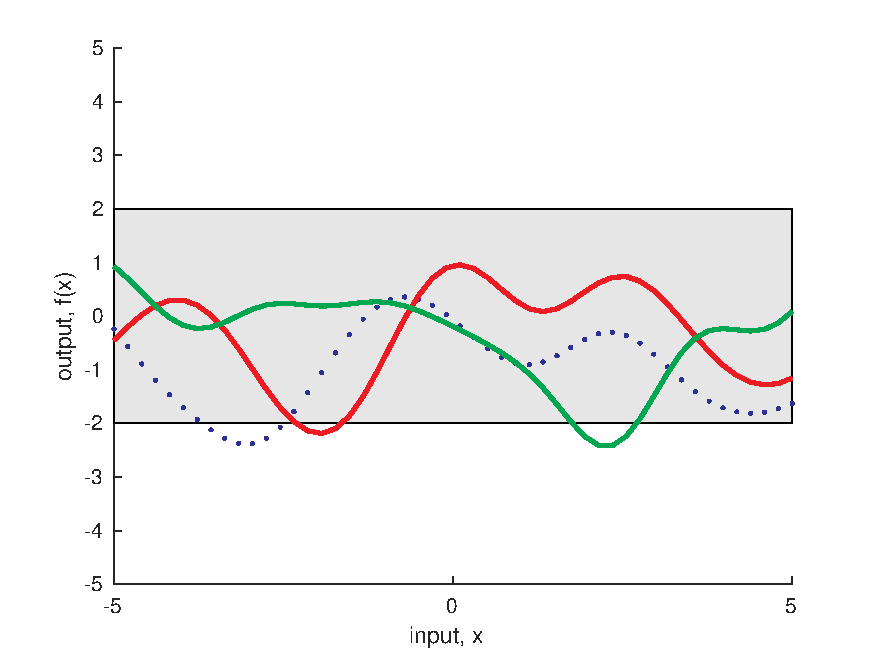
\includegraphics[width=.49\textwidth]{figures/prior_free.pdf}
	\hfill
	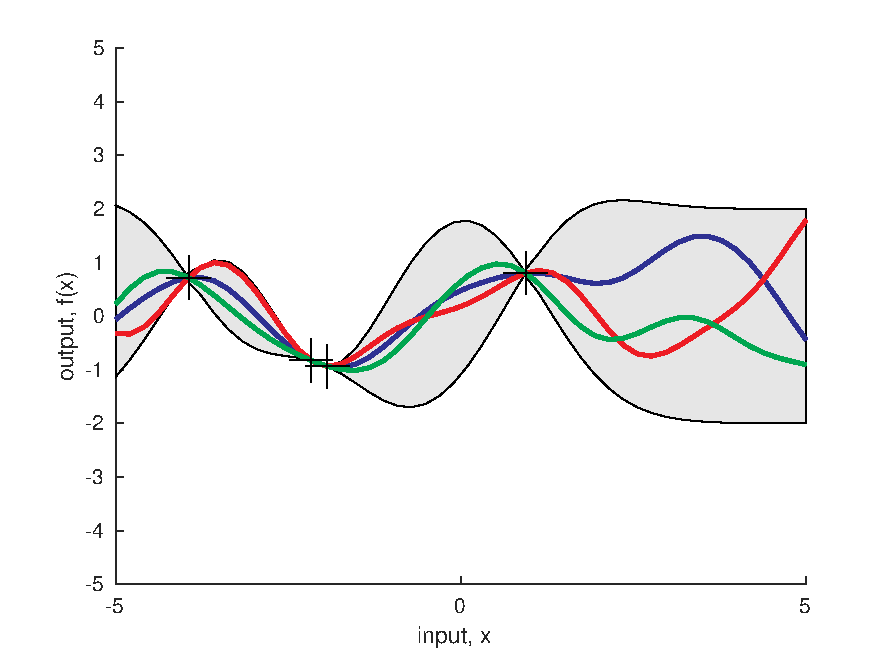
\includegraphics[width=.49\textwidth]{figures/posterior_free.pdf}
	\caption{Panel (a) shows three functions drawn at random from a GP prior; the dots indicate values of $y$ actually generated by GP; the two other functions (in red and green) have been drawn as lines by joining a large number of evaluated points. Panel (b) shows three random functions drawn from the posterior, i.e. the prior conditioned on
		the four noise free observations marked with cross symbols. In both plots the shaded area represents the
		pointwise mean plus and minus two times the standard deviation for each input value
		(corresponding to the 95\% confidence region), for the prior and posterior respectively.}
	\label{fig:noise_free}
\end{figure*}

\subsubsection{Predictions from noise free observations}
We are usually not primarily interested in drawing random functions from the prior, but want to incorporate the knowledge that the training data provides about the function. 
Initially, we will consider the simple special case where the
observations are \textit{noise free}, that is assume we are provided with a sample set:
\begin{equation*}
S=\{(x_i,f(x_i))\ |\ i=1,\ldots,n\}.
\end{equation*}
According to the GP prior, the joint distribution of the training outputs given by $f=(f_i)=(f(x_i))$, and the test outputs $f_∗=f(x_*)$ is defined by
\begin{equation}
\label{eq:noise_free}
\begin{bmatrix}
f\\ f_*
\end{bmatrix} \sim
\mathcal{N}\left(0,\ 
\begin{bmatrix}
K(X,X) & K(X,X_*)\\
K(X_*,X) & K(X_*,X_*)
\end{bmatrix}\right)
\end{equation}
If there are $n$ training points and $n_*$ test points then $K(X, X_*)$ denotes the $n \times n_*$ matrix of the covariances evaluated at all pairs of training and test points, and similarly for the other entries $K(X, X)\in\mathbb{R}^{n\times n}$, $K(X_*, X_*)\in\mathbb{R}^{n_*\times n_*}$ and $K(X_*, X)\in\mathbb{R}^{n_*\times n}$.

To get the posterior distribution over functions we need to restrict this joint prior distribution to contain only those functions which agree with the observed data points, i.e. we need to take conditional expectation.
The multivariate Gaussian distribution has the property that any conditional distribution is also Gaussian. Therefore, the distribution $f_* |X_*, X, f$ can be fully described with a mean and covariance matrix.
We can describe that mean and covariance using the standard multivariate Gaussian conditional formula:
\begin{lemma}
	Function values $f_*$ corresponding to test inputs $X_*$ can be sampled from the
	joint posterior distribution by evaluating the mean and covariance matrix as following:
	\begin{equation}
	\label{eq:samp_free}
	f_*| X_*,X,f \sim \mathcal{N}\left(K(X_*,X)K(X,X)^{-1} f,\quad 
	K(X_*,X_*)-K(X_*,X)K(X,X)^{-1}K(X,X_*)\right).
	\end{equation}
	\begin{proof}
		See Appendix~\ref{firstappendix}.
	\end{proof}
\end{lemma}
Figure~\ref{fig:noise_free}b shows the results of these computations given the four data points marked with cross symbols.

Note, that the formula~\eqref{eq:samp_free} is the same formula~\eqref{eq:mean} with $\Sigma_x=K(X_*,X_*)$, $\Sigma_{xy} = K(X_*,X)$, $\Sigma_y=K(X,X)$.


\subsubsection{Predictions from noisy observations}
It is typical for more realistic modeling situations that we do not have access to function values $f(x)$ themselves, but only noisy versions of the form $y=f(x)+\eps$. Assuming additive independent identically distributed Gaussian noise, $\eps\overset{i.i.d}{\sim}\mathcal{N}(0,\sigma_n^2)$, then the prior on the noisy observations becomes
\begin{equation}
\cov(y_p,\,y_q)= k(x_p,\, x_q))+\sigma_n^2 \delta_{pq}
\end{equation}
where $\delta_{pq}$ is a Kronecker delta which is one iff $p=q$ and zero otherwise. Equivalently, using the matrix notation the above equation can be written as
\begin{equation}
\cov(y)= k(X,\, X)+\sigma_n^2 I
\end{equation}
It follows from the independence assumption about the noise, that a diagonal matrix is added, in comparison to the noise free case, eq.~\eqref{eq:cov_free}.
Introducing the noise term in eq.~\eqref{eq:noise_free} we can write the joint distribution of the observed target values and the function values at the test locations under the prior as
\begin{equation}
\begin{bmatrix}
y\\ f_*
\end{bmatrix} \sim
\mathcal{N}\left(0,\ 
\begin{bmatrix}
K(X,X)+\sigma_n^2 I & K(X,X_*)\\
K(X_*,X) & K(X_*,X_*)
\end{bmatrix}\right)
\end{equation}
Deriving the conditional distribution corresponding to eq.~\eqref{eq:samp_free} we arrive at
the key predictive equations for Gaussian process regression
\begin{equation}
\label{eq:samp_noise}
\begin{aligned}
f_*| X_*,X,y \sim \mathcal{N}&\left(\bar{f}_*, \cov(f_*)\right),\quad\text{where} \\
\bar{f}_* &=\mu_{f_*} = K(X_*,X)\left[K(X,X)+\sigma_n^2 I\right]^{-1} y\\
\cov(f_*) &= K(X_*,X_*)-K(X_*,X)\left[K(X,X)+\sigma_n^2 I\right]^{-1} K(X,X_*)
\end{aligned}
\end{equation}

\begin{figure*}[h]
	\centering
	\includegraphics[width=.49\textwidth]{figures/posterior_noise02.pdf}
	\hfill
	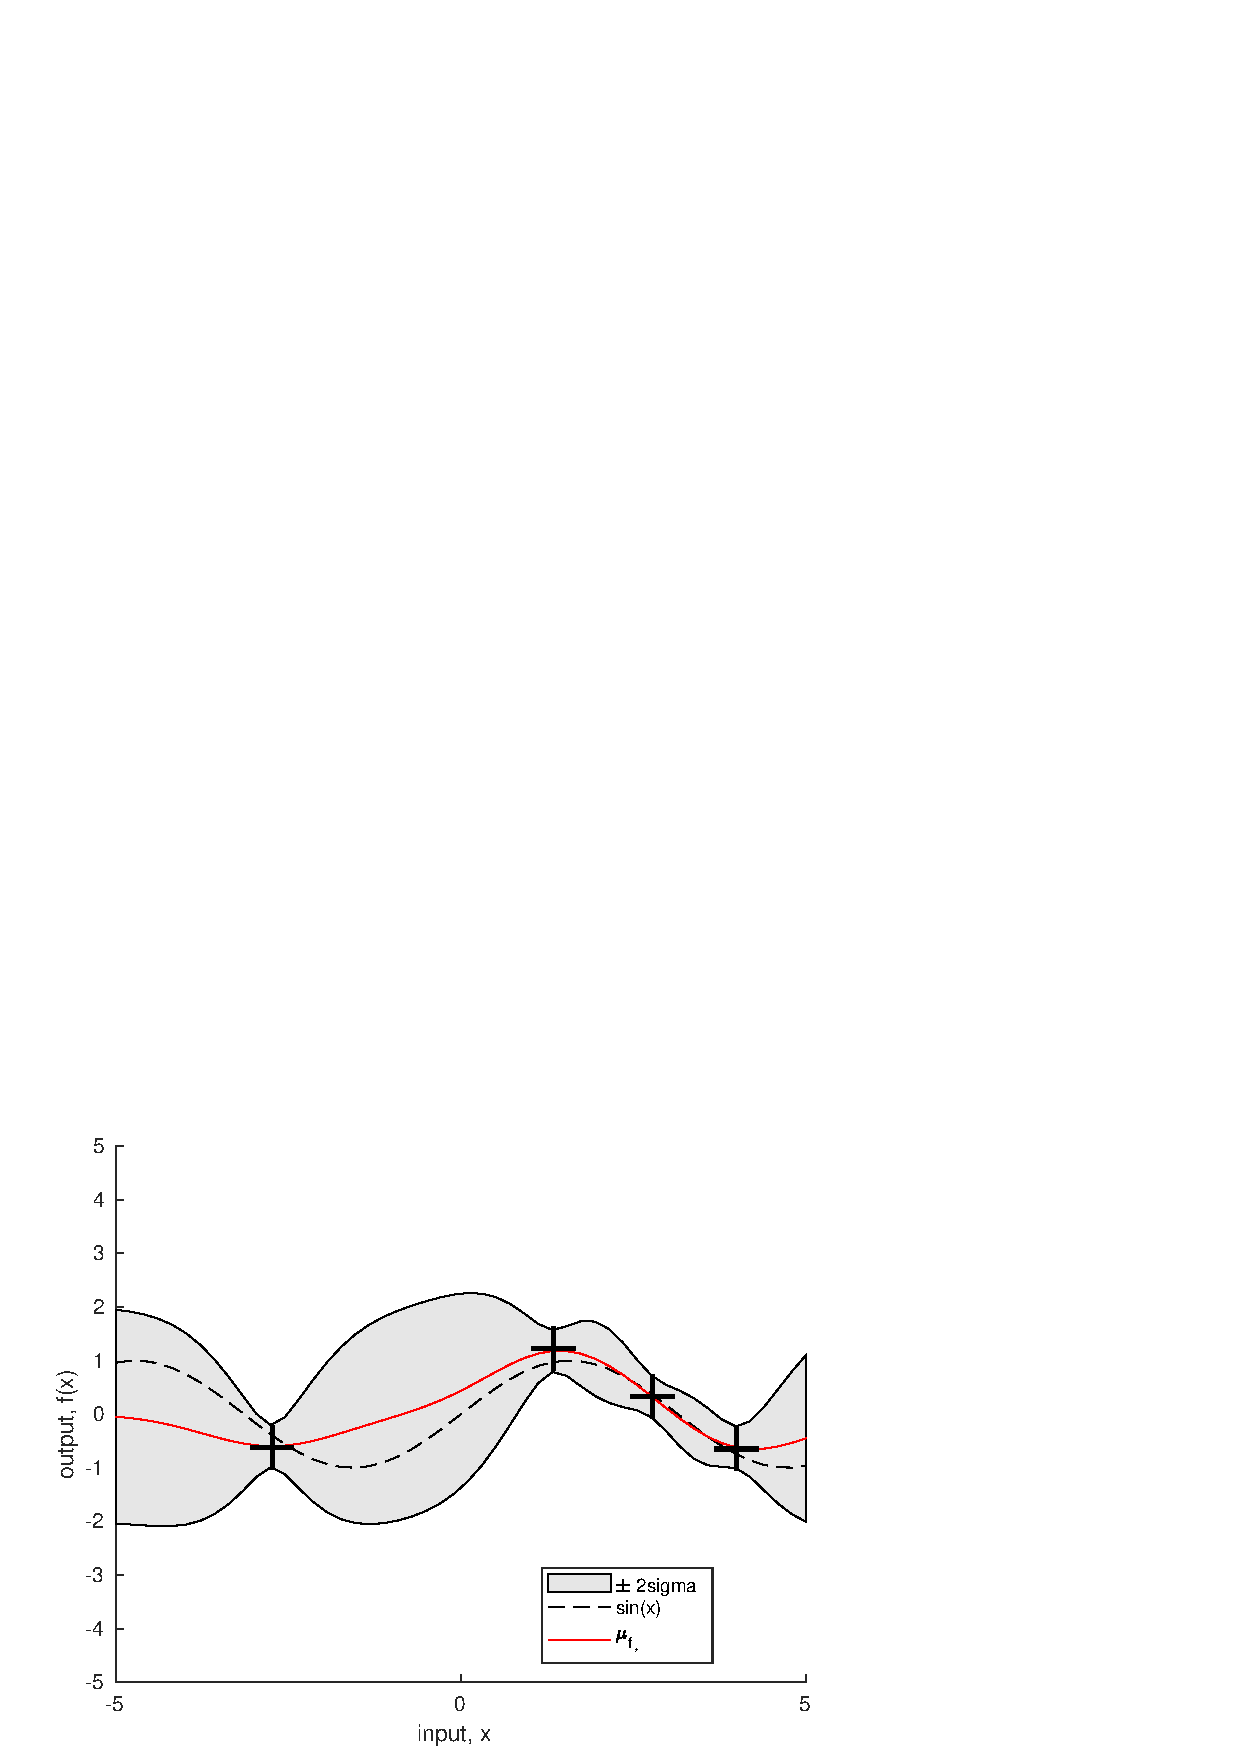
\includegraphics[width=.49\textwidth]{figures/posterior_noise02_true_mean.pdf}
	\caption{Observations with noise, $\sigma_n=0.2$: Panel (a) shows three random functions drawn from the noisy posterior, i.e. the prior conditioned on the four observations with noise marked with cross symbols. Panel (b) shows the underlying signal $\sin(x)$ and the predicted mean $\bar{f}_*$ signal.}
	\label{fig:noisy02}
\end{figure*}

\begin{figure*}[h]
	\centering
	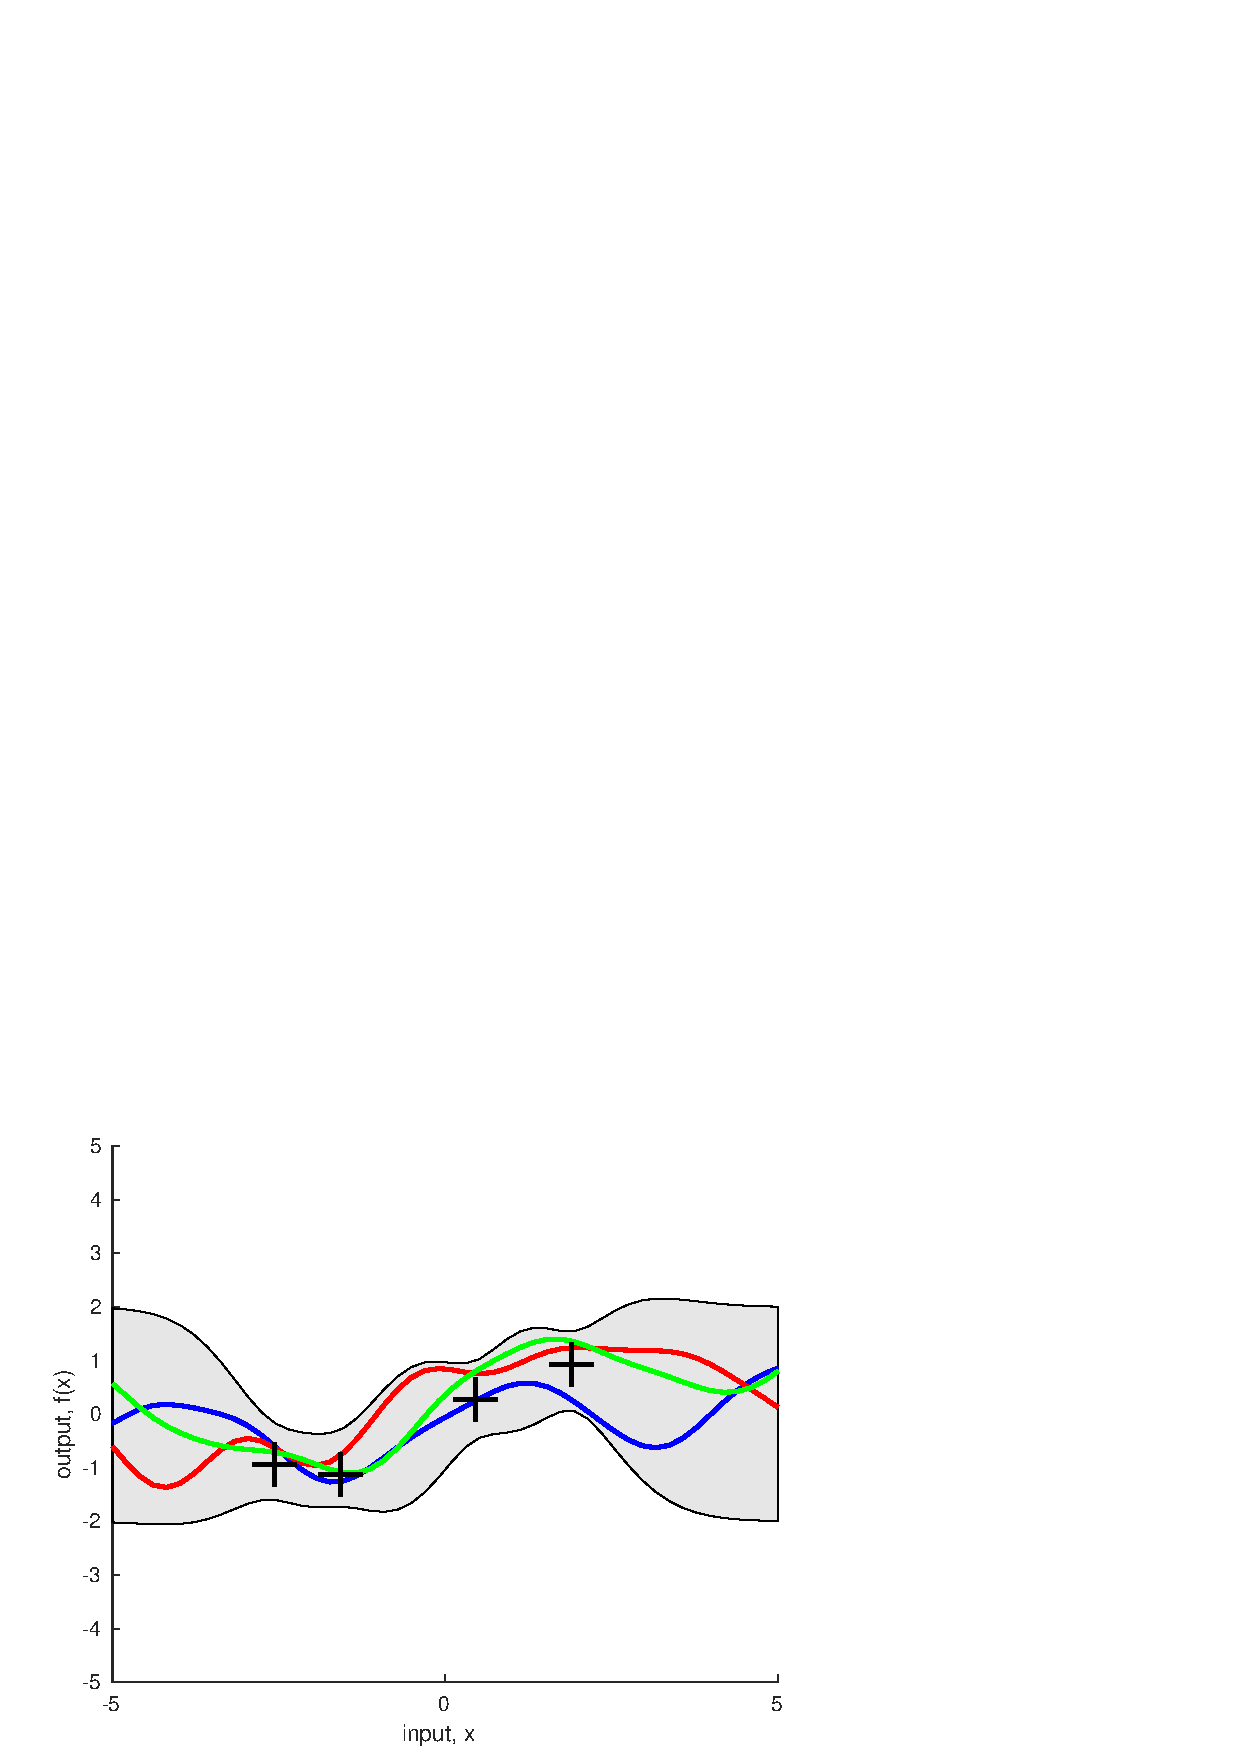
\includegraphics[width=.49\textwidth]{figures/posterior_noise04.pdf}
	\hfill
	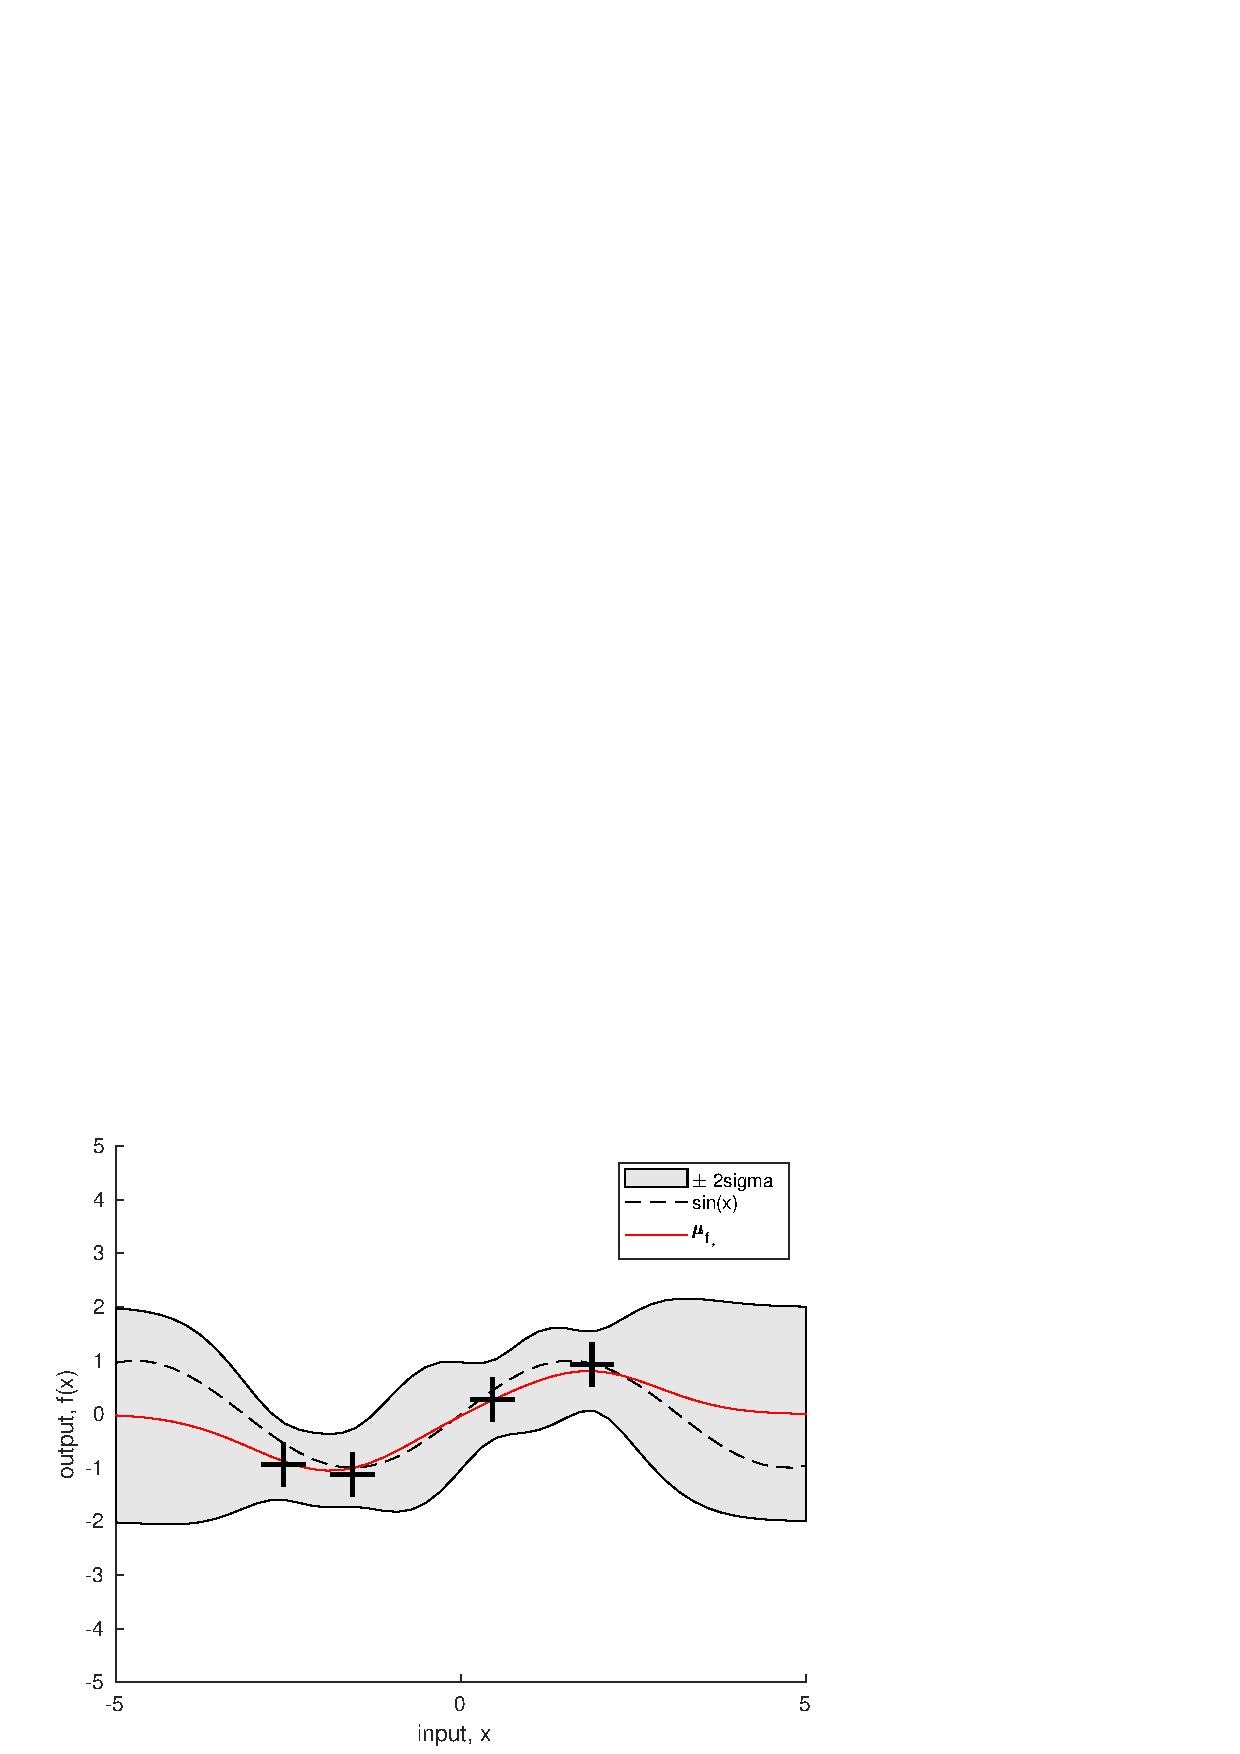
\includegraphics[width=.49\textwidth]{figures/posterior_noise04_true_mean.pdf}
	\caption{Observations with noise, $\sigma_n=0.4$: Panel (a) shows three random functions drawn from the noisy posterior, i.e. the prior conditioned on the four observations with noise marked with cross symbols. Panel (b) shows the underlying signal $\sin(x)$ and the predicted mean $\bar{f}_*$ signal.}
	\label{fig:noisy04}
\end{figure*}

Consider the data given by $y=f(x)+\eps$ for $\sigma_n=0.2$ in a Figure~\ref{fig:noisy02} and $\sigma_n=0.4$ in a Figure~\ref{fig:noisy04}, correspondingly. 
Subplot (a) in both figures present three realizations from posterior distribution, and subplot (b) draws the underlying signal $f(x)=sin(x)$ and predicted mean signal $\mu_{f_*}$.
The figures also show the 2 standard-deviation error bars. Notice how the error bars get larger in sampled points as the variance $\sigma_n$ gets higher ($\sigma_n=0.2$ in Figure~\ref{fig:noisy02} in comparison with $\sigma_n=0.4$ in Figure~~\ref{fig:noisy04}).

Note that the variance in eq.~\eqref{eq:samp_noise} does not depend on the observed targets $y$, but only on the inputs $X$ and $X_*$. This is a property of the Gaussian distribution.
The variance is the difference between two terms: the first term $K(X_*, X_*)$ is simply the prior covariance. From that is subtracted a (positive) term, representing the information the observations gives us about the function. 
We can very simply compute the predictive distribution of test targets $y_*$ by adding $\sigma_n^2 I$ to the variance in the expression for $\cov(f_*)$.


Let us now examine $f_*$ evaluated at a single test point $x_*$. Then $K(x_*,X)$ is a vector $[k(x_*,x_i)]_{i=1,\ldots,n}$ and
\begin{equation}
\label{eq:mean}
\bar{f}_*(x_*)=\sum\limits_{i=1}^n \alpha_i k(x_*,x_i),
\end{equation}
for $\alpha=[K(X,X)+\sigma_n^2I]^{-1}y$.
So it as a linear combination of $n$ kernel functions, each one centered on a training point.
The fact that the mean prediction for $f(x_*)$ can be
written as eq.~\eqref{eq:mean} despite the fact that the GP can be represented in terms of a possibly infinite number of basis functions is one manifestation of the
\textit{representer theorem}, see Section $6.2$ in~\cite{rasmussen:williams:2006}.
\subsection{Gaussian Process Regression as Linear Smoother}
GP regression aims to reconstruct the underlying signal $f$ by removing the contaminating noise $\eps$\footnote{This section was adapted from Section 2.6 in~\cite{rasmussen:williams:2006}.}.
To do this it computes a weighted average of the noisy observations $y$ as
\begin{equation}
\bar{f}_*(x_*) = k(x_*)^\top (K+\sigma_n^2 I)^{-1}y
\end{equation}
as $\bar{f}_*(x_*)$ is a linear
combination of the $y$ values, GP regression is a \textit{linear smoother}~\cite{Hastie90generalizedadditive}.

The predicted mean values $\bar{\mathbf{f}}$ at the training points are given by
\begin{equation}
\bar{\mathbf{f}}=K(K+\sigma_n^2 I)^{-1}y,\quad\text{for}\ K=K(X,X)
\end{equation}
Let K have the eigendecomposition
\begin{equation}
K = \sum\limits_{i=1}^{n} \lambda_i \mathbf{u}_i\mathbf{u}_i^\top
\end{equation}
where $\lambda_i$ is the $i$-th eigenvalue and $\mathbf{u}_i$ is the corresponding eigenvalue. 
As $K$ is real and symmetric positive semidefinite, its eigenvalues are real and non-negative, and its
eigenvectors are mutually orthogonal.
Let $\mathbf{y}=\sum_{i=1}^{n}\gamma_i \mathbf{u}_i$ for some coefficients $\gamma_i=\mathbf{u}_i^\top \mathbf{y}$. Then
\begin{equation}
\bar{\mathbf{f}}=\sum\limits_{i=1}^n \frac{\gamma_i \lambda_i}{\lambda_i+\sigma_n^2}\mathbf{u}_i.
\end{equation}
Note that
\begin{itemize}[noitemsep,topsep=0pt]
	\item if $\lambda_i \ll \sigma_n^2$ then summand term $\approx 0$, so the component in $\mathbf{y}$ along $\mathbf{u}_i$ is effectively	eliminated.
	\item if $\lambda_i \gg \sigma_n^2$ then summand term $\approx 1$, so the component is \textbf{not} eliminated.
\end{itemize}
Therefore, for most covariance functions that are used in practice the eigenvalues are larger for more slowly varying eigenvectors (e.g. fewer zero-crossings). This means that high-frequency components in $\mathbf{y}$ are smoothed out.
It acts as a filter, letting through only those ``terms above the noise''.


\section{Non-zero mean GPs: Incorporating Explicit Basis Functions}
It is common but not necessary to consider GPs with a zero mean function\footnote{This section was adapted from Section 2.7 in~\cite{rasmussen:williams:2006}.}. Note that this is not necessarily a drastic limitation, since the mean of the
posterior process is not confined to be zero. Yet there are several reasons why
one might wish to explicitly model a mean function. The use of explicit basis functions is a way to specify a \textit{non-zero mean} over functions.

Using a \textit{fixed} (deterministic) mean function $m(x)$ is trivial: Simply apply
the usual zero mean GP to the \textit{difference} between the observations and the
fixed mean function. With
\begin{equation}
f(x)\sim \mathcal{GP}(m(x),\ k(x,x')) 
\end{equation}
the predictive mean becomes
\begin{equation}
\bar{f}_* = m(X_*) + K(X_*,X)\left[K(X,X)+\sigma_n^2 I\right]^{-1} (y-m(X))
\end{equation}
and the predictive variance $\cov(f_*)$ remains unchanged from
eq.~\eqref{eq:samp_noise}.

However, in practice it can often be difficult to specify a fixed mean function.
In many cases it may be more convenient to specify a few fixed basis functions,
whose coefficients, $\beta$, are to be inferred from the data. Consider
\begin{equation}
\label{eq:non_zero}
g(x) = f(x) = h(x)^\top \beta,\quad\text{where}\quad
f(x)\sim\mathcal{GP}(0,\,k(x,x')),
\end{equation}
here $f(x)$ is a zero mean GP, $h(x)$ are a set of fixed basis functions (for example, polynomial $h(x)=(1,x,x^2,\ldots)$), and $\beta$ are
additional parameters. This formulation expresses that the data is close to a
global linear model with the residuals being modelled by a GP.
When fitting the model, one could optimize over the parameters $\beta$ jointly with
the hyperparameters of the covariance function. Alternatively, if we take the prior on $\beta$ to be Gaussian, $\beta\sim\mathcal{N}(b,B)$, we can also integrate out these
parameters. Following~\cite{o1978curve}, the obtained GP is
\begin{equation}
g(x) \sim\mathcal{GP}(h(x)^\top b,\ 
k(x,x')+h(x)^\top Bh(x')).
\end{equation}
The contribution in the covariance function caused by the uncertainty in the parameters of the mean.
If we plug in the mean and covariance functions of $g(x)$ into eq.~\eqref{eq:non_zero} and
$\eqref{eq:samp_noise}$, we obtain
\begin{align}
\bar{g}(X_*) &= H_*^\top \bar{\beta}+
K_*^\top K_y^{-1}(y-H^\top \bar{\beta})=
\bar{f}(X_*)+R^\top \bar{\beta},\label{eq:non-zero_mean}\\
\cov(g_*) &= \cov(f_*) + R^\top (B^{-1} + H K_y^{-1}H^\top)^{-1} R\label{eq:non-zero_cov}
\end{align}
where the $H$ matrix collects the $h(x)$ vectors for all training cases, $H_*$ collects all test points, and $\bar{\beta}$ and $R$ are defined as
\begin{equation}
\begin{aligned}
\bar{\beta} &= (B^{-1} + H K_y^{-1}H^\top)^{-1} (H K_y^{-1}y + B^{-1}b)\\
R &= H_* - H K_y^{-1}K_*.
\end{aligned}
\end{equation}
The interpretation of the mean expression $\bar{\beta}$ , eq.~\eqref{eq:non-zero_mean}: is
the mean of the global linear model parameters, being a compromise between
the data term and prior, and the predictive mean is simply the mean linear
output plus what the GP model predicts from the residuals. The covariance $\cov(g_*)$, eq.~$\eqref{eq:non-zero_cov}$, is
the sum of the usual covariance term $\cov(f_*)$ and a new non-negative contribution.

Exploring the limit of the above expressions as the prior on the $\beta$ parameter becomes vague, $B^{-1}\to O$ (where $O$ is the matrix of zeros), we obtain a
predictive distribution which is independent of $b$
\begin{align}
\bar{g}(X_*) &=
\bar{f}(X_*)+R^\top \bar{\beta},\\
\cov(g_*) &= \cov(f_*) + R^\top (H K_y^{-1}H^\top)^{-1} R,
\end{align}
where the limiting $\bar{\beta}= (H K_y^{-1}H^\top)^{-1} H K_y^{-1}y$.



% Uncomment for bibliography
\newpage
\bibliographystyle{abbrvnat}
\bibliography{refs_lecture24}

\newpage
\appendix
\section{Appendix}
\subsection{Partitioned Gaussian Densities}\label{firstappendix}
\begin{theorem}\cite{schon2011manipulating}
	Let the random vector $x$ be Gaussian $x~\sim\mathcal{N}(\mu,\Sigma)$ with mean and variance as following
	\begin{equation}
	\mu = \begin{bmatrix}
	\mu_a\\ \mu_b
	\end{bmatrix},
	\quad
	\Sigma = \begin{bmatrix}
	\Sigma_{aa} & \Sigma_{ab} \\
	\Sigma_{ab}^\top & \Sigma_{bb}
	\end{bmatrix},
	\end{equation}
	then the conditional density $p(x_a | x_b)$ is given by 
	\begin{equation}
	p(x_a|x_b) = \mathcal{N}(\mu_{a|b},\, \Sigma_{a|b},)
	\end{equation}
	where 
	\begin{align}
	\mu_{a|b}&=\mu_a + \Sigma_{ab} \Sigma_{bb}^{-1} (x_b - \mu_b) \\
	\Sigma_{a|b} &=\Sigma_{aa} - 
	\Sigma_{ab} \Sigma_{bb}^{-1}\Sigma_{ab}^\top
	\end{align}
	\begin{proof}
		We will make use of the fact that 
		\begin{equation}
		p(x_a | x_b) = \frac{p(x_a,x_b)}{p(x_b)}
		\end{equation}
		which is according to the definition of the normal distribution (see eq.\eqref{eq:gaus_var}) is
		\begin{equation}
		\label{eq:p}
		p(x_a|x_b) = \frac{\sqrt{\det\Sigma_{bb}}}{(2\pi)^{n_a/2} \sqrt{\det \Sigma}} \exp(E)
		\end{equation}
		\begin{equation}
		\label{eq:e}
		E = -\frac{1}{2}(x-\mu)^{\top} \Sigma^{-1} (x-\mu) -
		\frac{1}{2}(x_b-\mu_b)^{\top} \Sigma_{bb}^{-1} (x_b-\mu_b)
		\end{equation}
		Since 
		\begin{equation}
		\det\Sigma = \det \begin{pmatrix}
		\Sigma_{aa} & \Sigma_{ab}\\ \Sigma_{ab}^\top & \Sigma_{bb}
		\end{pmatrix} = 
		\det \Sigma_{bb} \det (\Sigma_{aa}- \Sigma_{ab}\Sigma_{bb}^{-1} \Sigma_{ab}^\top)
		\end{equation}
		the constant in front of the exponential in~\eqref{eq:p} results in the following expression
		\begin{equation}
		\label{eq:const}
		  \frac{\sqrt{\det\Sigma_{bb}}}{(2\pi)^{n_a/2} \sqrt{\det \Sigma}} = 
		 \frac{1}{(2\pi)^{n_a/2} \sqrt{\det (\Sigma_{aa}- \Sigma_{ab}\Sigma_{bb}^{-1} \Sigma_{ab}^\top)}} = 
		 \frac{1}{(2\pi)^{n_a/2} \sqrt{\det \Lambda_{aa}^{-1}}}
		\end{equation}
		The precision
		matrix $E$, eq.~\eqref{eq:e}, is given by
		\begin{align*}
		E &= -\frac{1}{2}(x-\mu)^{\top} \Lambda (x-\mu) -
		\frac{1}{2}(x_b-\mu_b)^{\top} \Sigma_{bb}^{-1} (x_b-\mu_b) = \\
		& = 
		-\frac{1}{2}(x_a-\mu_a)^{\top} \Lambda_{aa} (x_a-\mu_a) -
		\frac{1}{2}(x_a-\mu_a)^{\top} \Lambda_{ab}^{-1} (x_b-\mu_b)-\\ 
		&\quad-
		\frac{1}{2}(x_b-\mu_b)^{\top} \Lambda_{ba}^{-1} (x_a-\mu_a) 
		-
		\frac{1}{2}(x_b-\mu_b)^{\top} (\Lambda_{bb}-\Sigma_{bb}^{-1}) (x_b-\mu_b) 
		=\\
		&= 
		-\frac{1}{2}x_a^{\top} \Lambda_{aa} x_a + 
		x_a^\top (\Lambda_{aa}\mu_a -\Lambda_{ab}(x_b-\mu_b) ) - \\
		&\quad - \frac{1}{2}\mu_a^{\top} \Lambda_{aa} \mu_a + 
		\frac{1}{2}\mu_a^{\top} \Lambda_{ab} (x_b-\mu_b) - 
		 \frac{1}{2}(x_b-\mu_b)^\top (\Lambda_{bb}-\Sigma_{bb}^{-1})(x_b-\mu_b).
		\end{align*}
		Using the block matrix inversion result
		\begin{equation}
		\Sigma_{bb}^{-1} \Lambda_{bb} - \Lambda_{ba} \Lambda_{aa}^{-1} \Lambda_{ab}
		\end{equation}
		and completing the squares results in 
		\begin{equation}
		\label{eq:E}
		E = -\frac{1}{2} (x_a - (\Lambda_{aa}\mu_a - \Lambda_{ab}(x_b-\mu_b)))^\top
		\Lambda_{aa} 
		(x_a - (\Lambda_{aa}\mu_a - \Lambda_{ab}(x_b-\mu_b)))
		\end{equation}
		Finally,  combining~\eqref{eq:const}and \eqref{eq:E} results in
		\begin{equation}
		p(x_a|x_b) = 
		 \frac{1}{(2\pi)^{n_a/2} \sqrt{\det \Lambda_{aa}^{-1}}} \exp(E)
		\end{equation}
		which concludes the proof.
	\end{proof}
\end{theorem}
 \end{document}






